
\section{Integrated Mission Simulation and DITL Supporting Analysis}\label{app:ditl-detail}
\subsection{Purpose and Source}\label{app:ditl-source}
The integrated model in \texttt{src/simulations/ditl/ANTARA\_Science\_Sim.py} combines orbit propagation, spacecraft attitude, electrical power, mode transitions, proton-environment assumptions and detector accumulation, and ground-station communications. Its current implementation is a simulation model, not a hardware-in-the-loop qualification system. The shared configuration and individual presets are documented in Appendix~\ref{app:sim-provenance}.
\subsection{Defined Mission Scenarios}\label{app:ditl-preset-details}
The source defines \texttt{leop\_24h}, \texttt{no\_leop\_24h} and \texttt{leop\_1yr}. The first includes Cold and Dark and Detumble; the second begins in Sun Pointing without LEOP startup; the annual scenario includes startup over 8,760 hours. Command-line values may override preset defaults. A comparison of the three scenarios is meaningful only when each output is accompanied by its exact version and configuration.
\subsection{Mode Execution, Time and Energy}\label{app:ditl-accounting}
During startup, detumble and slewing, the simulator uses its fine time cadence. Other operating modes may use a coarser step. Mode occupancy, energy use, detector accumulation and mission elapsed time advance with the same actual integration interval. The interval length is recorded in \texttt{interval\_duration\_sec}; the last zero-duration terminal telemetry row should not be counted as additional mission time. Reported fractions should therefore use total elapsed time, not raw row fractions.
The ADCS model retains finite slew and settling requirements, momentum saturation handling and recovery logic. During saturation hold, scientific collection and downlink transmission are inhibited in the documented model. The end of a planned slew duration is not by itself proof of achieved target alignment.
\subsection{Science Data, Detector Statistics and Model Limits}\label{app:ditl-science}
The detector model accumulates expected bin counts and serializes histograms into science data separately. An interval with accepted events need not produce a positive new packet volume until a flush. SAA-exit and simulation-horizon flushes belong to the corresponding pass totals. Bin precision estimates use $1/\sqrt{N}$ for accumulated expected counts, but this does not represent calibrated detector response, stochastic-count realization or a fully validated low-count confidence interval. The environment model's legacy AP9-named variable is a configured baseline and not an independent AP9 computation.
\subsection{Adopted Annual-Labelled Evidence}\label{app:ditl-evidence}
At the team's direction, the short 24h-named exports are excluded from the operational comparison. Only the \texttt{leop\_1yr} group is used here. Its telemetry is incomplete at 50 days plus 20~s; its event exports reach nearly 365 days but are not a matching completion record. Table~\ref{tab:annual-ditl} summarizes telemetry contents. Exact hashes and separate artifact manifests prevent those series being pooled into an apparently complete run. The model's recorded minimum battery is 15.21520~Wh (60.8608\% of the 25~Wh planning reference); this is not an annual worst-case bound.

\subsection{Exposure, Storage and Event Reconciliation}
For the incomplete annual telemetry, total accounted time is 4\,320\,020~s; geometric SAA time is 130\,664~s; Detection-labelled SAA time is 1246~s; acquisition-gate time is 342~s. Thus model acquisition/SAA is $342/130664=0.26174\%$, not the historical detection-conditional 62.7\% fraction. Accepted physical detector exposure, reconstructed proton measurements and delivered current-FPDU records remain unqualified. Repeated time samples are not independent passages.

The 64-bin expected-count arrays conserve summed rate-times-exposure within text precision (maximum per-record residual $1.21\times10^{-7}$ counts); periphery merging moves counts between bins and still requires effective-edge metadata validation. Legacy five-layer efficiencies and assumed dead time do not apply to the current payload. Histogram totals are model expectations, not calibrated event reconstructions.

Cumulative generated and transferred columns close with incremental telemetry totals. Storage satisfies initial 10 plus generation minus transfer within $1.8\times10^{-15}$ source MB, peaking at 10.00492859 and ending at 10. The histogram-byte column omits 1088 bytes relative to binary-converted generation totals; four serialization rows outside acquisition are consistent with boundary flushes, not automatically lost events. Packet contents and ground receipt cannot be checked without packet archives. MB/MiB conventions require correction before byte-accurate RF accounting.
\begin{figure}[H]\centering\includegraphics[width=.9\linewidth]{evidence/science-ditl/figures/partial_annual_storage.png}
\caption{Telemetry-only storage and cumulative transfer in the incomplete annual-labelled artifact. Event exports disagree even within this horizon and are excluded from these curves.}\label{fig:partial-storage}\end{figure}

\begin{table}[H]\centering\small
\caption{Overlap consistency check, through 4\,320\,020~s; outputs are not accepted as one reconciled run.}\label{tab:annual-overlap}
\begin{tabularx}{\linewidth}{@{}Xrr@{}}\toprule Metric & Telemetry & Event exports\\\midrule
SAA dwell (s) & 130664 & 120568\\
Contact visibility/duration (s) & 36754 & 33668\\
Transferred (source MB) & 0.004929 & 0.477814\\
Science generation / SAA attribution (source MB) & 0.004929 & 0.396622\\
Legacy expected counts & $2.51815\times10^7$ & $4.24178\times10^8$\\
Slewing (s) & 3616666 & 67844\\\bottomrule
\end{tabularx}\end{table}
Full event exports contain 820 contacts and extend nearly 365 days, but lack a matching complete telemetry series and completion manifest. Their 2000-03-01 UTC origin is historical, not 2029 calibration. These discrepancies block annual performance claims.

\subsection{Historical Detumble Summary}\label{app:detumble-evidence}
The supplied 50\,000-row summary reports 16\,133 successful trials and 33\,867 nonconverged trials; all unsuccessful completion times are infinite. Successful-only median, 95th percentile and maximum times are 951.5, 2569.0 and 3026.5~s. Whole-population convergence quantiles and flight reliability are not established. The first baseline row completes in 1009~s, distinct from the integrated 2460~s startup. Initial spin magnitudes range from approximately 0.0008 to 60~deg/s. All rows specify nonzero initial accelerations; the current source rejects that independent-acceleration model, preventing exact reproduction with current code.
\begin{figure}[H]\centering\includegraphics[width=\linewidth]{evidence/detumble/figures/validated_summary.png}
\caption{Historical detumble summary. The empirical completion curve retains all 50\,000 rows as denominator; it is not a censor-adjusted survival estimate. Spin-bin proportions do not establish flight initial-condition probabilities.}\label{fig:detumble-summary}\end{figure}
The summary marks 25\,473 rate-cap hits and records zero peak wheel momentum in every row; neither establishes actuator adequacy. Initial attitude distribution, magnetic field, gains, source revision, random seeds, timeout and failure reasons are missing. No angular-rate or control-effort histories are supplied. Close the generating model and censoring record before bounded timestep, field-orientation, torque/momentum and coupled acquisition validation. Retain reaction wheels plus magnetorquers; no CMG configuration is inferred.

\subsection{Science Record v3 Queue Diagnostic}\label{app:v3-queue}
The new reference calculation uses only recorded visibility intersect Relay for service, at the full 19.2~kbps and initially empty science queue. Ideal reading exits generate record slots; no actual integer detector counts are fabricated. The preferred MMSC/MSC/EMSC cases generate and transfer 16\,644/50\,808/67\,452 bytes respectively, with zero final backlog in this incomplete trace. Maximum queues equal these totals before delivery. The historical initial 10 source-MB store is not silently included as new v3 science.

\begin{figure}[H]\centering
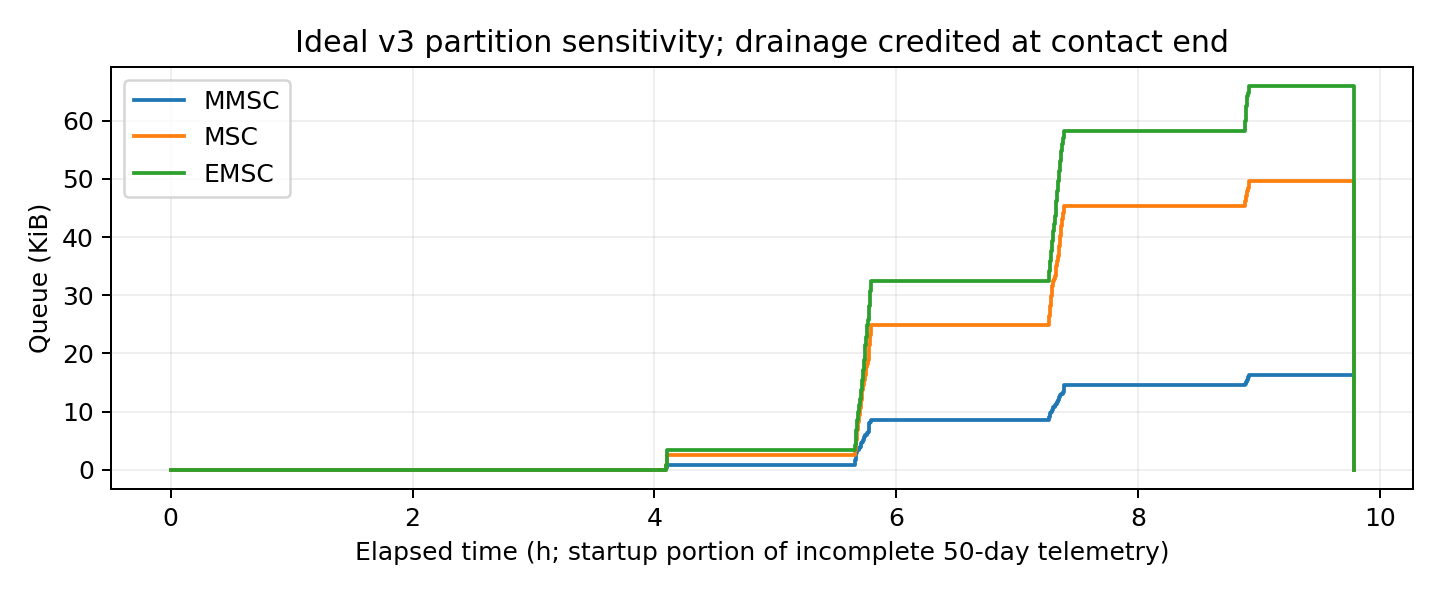
\includegraphics[width=\linewidth]{data/derived/telemetry_v3_2026-11-09/bounded_queue.png}
\caption{Time-aligned record-slot sensitivity using legacy acquisition gates. Display credits drainage at eligible contact end; exact byte-balance calculations service queued bytes during contact. The plot is not observed v3 telemetry or qualified science production.}\label{fig:v3-queue}
\end{figure}
Every release and service window has an auditable ledger: queue before, transferred bytes, remaining queue and unused ideal capacity. The longest sampled Relay gap (48\,456~s) contains no generation in this trace; it does not determine the maximum backlog. Missed-window and 1/3/7-day outages preserve the same finite peak because acquisition subsequently remains disabled. The unusually small horizon-specific data-balance rates must not be used to downsize the radio. Record validity does not require individual Poisson precision; zero-count exposures remain records, while science-tier success depends on accumulated qualified measurements and independent passages. Current payload response and sustained production remain unverified.
